\section{Validation Strategy}

\subsection{Definition}
Regarding validation processes related to complex systems, \textcite{Oberkampf2010} suggested using a building block or system complexity hierarchy approach due to the infeasibility of true validation on most complex systems. 

This document adopts that hierarchical strategy, organizing model evaluation across progressively challenging scenarios, ranging from simplified geometries in controlled and simplified conditions to real-world urban environments. This allows to assess the accuracy of the computational results compared with the experimental data at multiple degrees of physics coupling and geometric complexity.\newline

Validation strategy decomposes the problem into subproblems of increasing complexity, exploiting the possible configurations of the ABL and the unitary problems concerning urban dispersion phenomena.\newline

Validation procedure takes into account available datasets related to atmospheric dispersion modelling in micro-scale environments. These validation data for numerical models must fulfil specific requirements with respect to completeness, spatial and temporal resolution, accuracy, representativeness, and the documentation of the measured results must be available \parencite{Chang2003}.

\subsection{Comparative analyses}

For each dataset, an OpenFOAM test case is developed to enable a consistent suite of comparative analyses. These analyses serve both general and case-specific purposes.\newline

\noindent
General objectives for all test cases include:
\begin{itemize}
    \item Performing grid sensitivity studies to assess numerical resolution dependence;
    \item Conducting sensitivity analyses on turbulence models and numerical schemes;
    \item Exploring transitions from full-order to reduced-order modeling approaches;
    \item Replacing experimental boundary conditions with reconstructed inflow profiles
\end{itemize}


\subsection{Assessment of the results}
Model performance is assessed by comparing simulation results to experimental datasets. The validation process focuses on:
\begin{itemize}
    \item Quantitative metrics comparing point-wise scalar values (e.g., velocity magnitude, temperature, pollutant concentration);
    \item Qualitative representation of results with 2D and 3D plots to aid interpretation and model comparison.
\end{itemize}

\noindent
Each test case includes the computation of statistical metrics, detailed in \ref{sec:statistical_metrics}. An example of the post-processing procedure is provided to illustrate the analysis of simulation results (see Section \ref{sec:post_processing}).

\subsubsection{Statistical metrics \label{sec:statistical_metrics}}
Quantitative comparison of experimental and model results is performed using the following statistical performance measures (where $P_i$ is the model prediction, $O_i$ is the observed value):
\begin{description}

    \item[Geometric mean bias $\;\left( MG \right)$ :] is the logarithmic measure of the mean relative bias thus is strongly influenced by extremely low observations and predictions for the concentrations.It is not so strongly influenced by infrequently occurring high observations and pre dictions for the concentrations as the fractional bias.It indicates only systematic errors. For an ideal model MG=1. 

    \begin{equation*}
        MG = \mbox{exp}\;(\,\frac{1}{n}\;\sum_{i=1}^n\mbox{ln} O_i - \frac{1}{n}\;\sum_{i=1}^n\mbox{ln} P_i\,)
    \end{equation*}

    \item[Geometric variance $\;\left( VG \right)$ :] is a metric like the NMSE, it shows the scatter in the data and therefore contains both, systematic and random errors. For an ideal model prediction one would have VG=1.

    \begin{equation*}
        VG\;=\;\mbox{exp}\,\left[\,\frac{1}{n}\;\sum_{i=1}^n(\mbox{ln}\,O_i - \mbox{ln}\,P_i)^2\,\right]
    \end{equation*}

    \item[Normalised mean square error $\;\left( NMSE \right)$ :] is a measure of the scatter of the data and therefore indicates both, systematic and random errors. For an ideal model prediction one would have NMSE=0. NMSE makes no sense for parameters that can take both positive and negative values, such as velocity components.

    \begin{equation*}
        NMSE\;=\;\frac{1}{n}\;\sum_{i=1}^n\;\frac{(\;O_i - P_i\;)^2}{\overline{O}\;\overline{P}}
    \end{equation*}

    \item[Normalised relative error $\;\left( NRE_i \right)$ :] is a local measure of the relative difference between predicted and observed values, computed at each spatial point $i$. It is typically used to generate visualisations, such as 3D error plots.

\begin{equation*}
    NRE_i = \left| \frac{P_i - O_i}{O_i} \right| \times 100
\end{equation*}

\end{description}

\clearpage

\subsubsection{Post-processing example \label{sec:post_processing}}

Here we provide an example of the basic post-processing available for each test case that belongs to the validation procedure.

\begin{table}[ht]
    \centering
    \begin{tabular}{r|cc|cc|cc}  
        \toprule
        \textbf{Case} & \multicolumn{2}{c|}{\textbf{NMSE}} & \multicolumn{2}{c|}{\textbf{MG}} & \multicolumn{2}{c}{\textbf{GV}} \\
                     & UMag & k                           & UMag & k                         & UMag & k \\
        \midrule
        Case-A & 0.030 & 1.342 & 1.013 & 2.067 & 1.262 & 2.761 \\
        Case-B & 0.030 & 1.341 & 1.011 & 2.067 & 1.264 & 2.763 \\
        Case-C & 0.023 & 1.603 & 0.991 & 2.266 & 1.251 & 3.462 \\
        Case-D & 0.027 & 1.345 & 1.012 & 2.087 & 1.252 & 2.845 \\
        Case-E & 0.034 & 1.297 & 0.964 & 2.035 & 1.227 & 2.907 \\
        \bottomrule
    \end{tabular}
    \caption{Tabular data of statistical metrics - Comparison of multiple
        simulations data at the end}
    \label{tab:statistics}
\end{table}

\begin{figure}[h!]
    \centering
    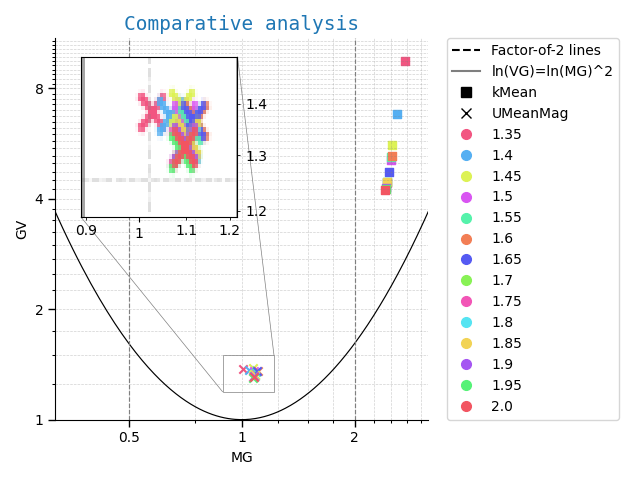
\includegraphics[width=0.9\textwidth]{imgs/quantitative_package_single.png}
    \caption{Graphical representation of statistical metrics - comparison of single 
        simulation data over time}
    \vspace*{-0.5cm}
    \label{example_quantitative} 
\end{figure}

\begin{figure}[h!]
    \centering
    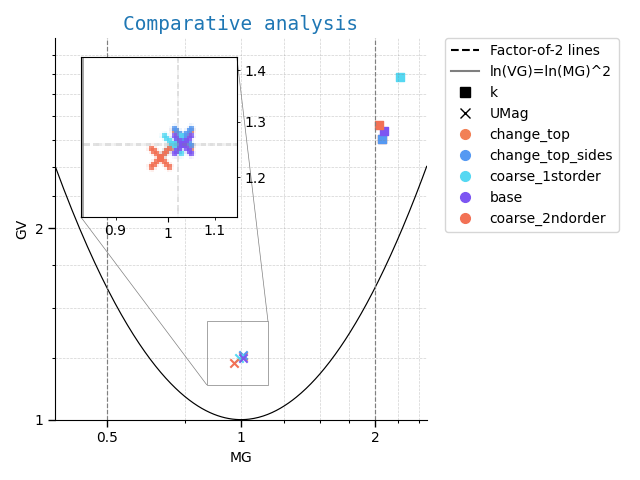
\includegraphics[width=0.9\textwidth]{imgs/quantitative_package_multi.png}
    \caption{Graphical representation of statistical metrics - Comparison of multiple
        simulations data at the end}
    \vspace*{-0.5cm}
    \label{example_quantitative} 
\end{figure}

\newpage

\begin{figure}[h!]
    \centering
    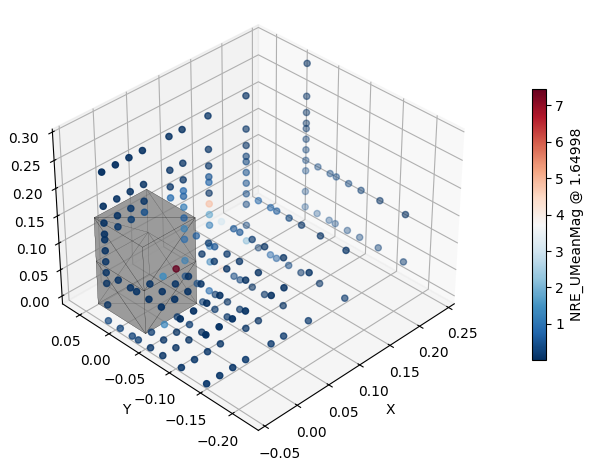
\includegraphics[width=0.8\textwidth]{imgs/3dplot_nre_example.png}
    \caption{3D plot of Normalised Relative Error (NRE)}
    \vspace*{-0.5cm}
    \label{example_3dplot}
\end{figure}

\begin{figure}[h!]
    \centering
    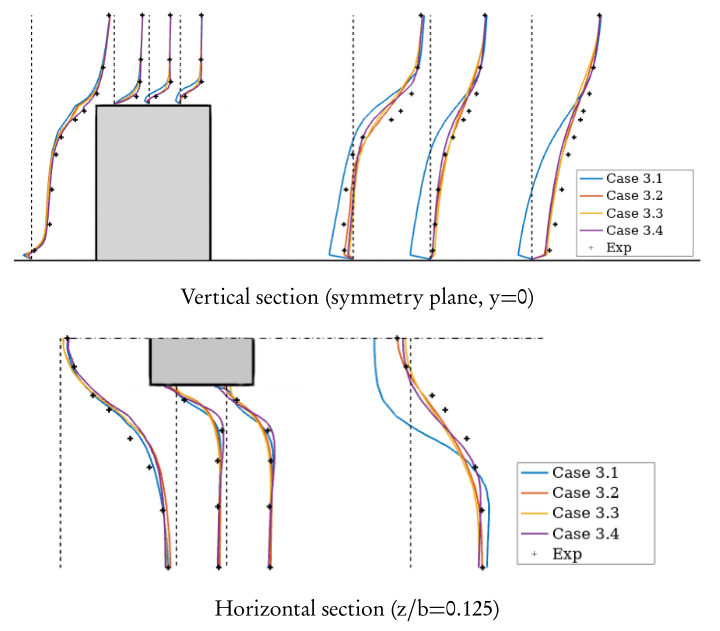
\includegraphics[width=1.0\linewidth]{imgs/qualitative_package.png}
    \caption{Comparison of multiple simulations results line data}
    \label{Line data visualization along with experiment point data}
\end{figure}


\clearpage

\subsection{Validation Strategy Diagram}
Here follow the proposed validation hierarchy with the up-to-date selected test cases to be simulated.
\vspace*{-1cm}
\begin{figure}[h!]
    \centering
    \begin{overpic}[width=\textwidth]{imgs/block_diagram.pdf}
        \put(7.8,30){\hyperlink{link:aij_A}{\makebox[3cm][l]{\rule{0pt}{0.5cm}}}}
        \put(7.8,26.3){\hyperlink{link:sef_A}{\makebox[3cm][l]{\rule{0pt}{0.5cm}}}}
        \put(7.8,22.5){\hyperlink{link:aij_C}{\makebox[3cm][l]{\rule{0pt}{0.5cm}}}}
        \put(7.8,19){\hyperlink{link:cost_c_wt}{\makebox[3cm][l]{\rule{0pt}{0.5cm}}}}
        \put(17.8,30){\hyperlink{link:tpu_A}{\makebox[3cm][l]{\rule{0pt}{0.5cm}}}}
        \put(17.8,26.3){\hyperlink{link:sef_A}{\makebox[3cm][l]{\rule{0pt}{0.5cm}}}}
        \put(17.8,22.5){\hyperlink{link:cost_m}{\makebox[3cm][l]{\rule{0pt}{0.5cm}}}}
        \put(31.8,30){\hyperlink{link:sef_A}{\makebox[3cm][l]{\rule{0pt}{0.5cm}}}}
        \put(31.8,26.3){\hyperlink{link:sef_A}{\makebox[3cm][l]{\rule{0pt}{0.5cm}}}}
        \put(50.8,30){\hyperlink{link:tpu_C}{\makebox[3cm][l]{\rule{0pt}{0.5cm}}}}
        \put(50.8,26.3){\hyperlink{link:sef_A}{\makebox[3cm][l]{\rule{0pt}{0.5cm}}}}
        \put(50.8,22.5){\hyperlink{link:sef_A}{\makebox[3cm][l]{\rule{0pt}{0.5cm}}}}
        \put(26,8){\hyperlink{link:cost_c_f}{\makebox[3cm][l]{\rule{0pt}{0.5cm}}}}
        \put(36,8){\hyperlink{link:turb_p}{\makebox[3cm][l]{\rule{0pt}{0.5cm}}}}
    \end{overpic}
    \vspace*{-1cm}
    \caption{Tiers representation of the validation strategy (All test cases refer to datasets described in the following sections, i.e. AIJ, TPU, SEF, COST, and TURB). }
    \label{validation_strategy} 
\end{figure}
